\section{Защитное время}
Помимо использования циклического префикса, описанного в предыдущем разделе, вводится параметр <<Защитного времени>> (ЗВ, Guard Time).
Рассмотрим систему, изображенную на рисунке ~\ref{fig:vol_mobile_cell}.
\begin{figure}[H]
    \centering
    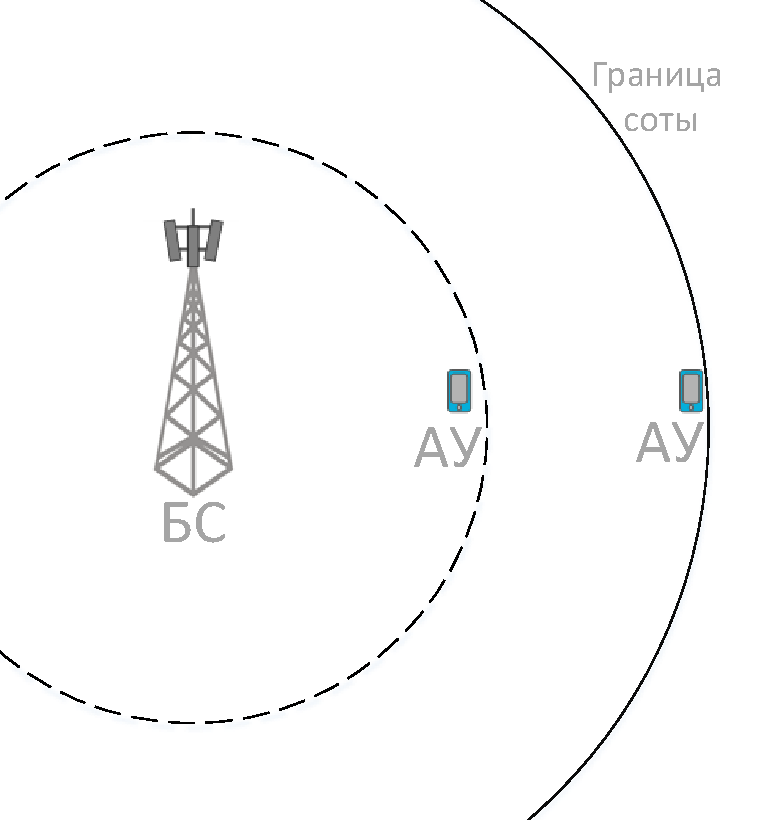
\includegraphics[width=0.5\textwidth]{img/vol_mobile_cell}
    \caption{Мобильная сота с двумя абонентами}
    \label{fig:vol_mobile_cell}
\end{figure}

Данная система состоит из базовой станции (БС) и двух абонентских устройств (АУ), одно из которых
расположено непосредственно у базовой станции, второе --- на границе соты. АУ, расположенное рядом с
БС, получит сообщение быстрее, чем АУ, расположенное на границе соты. Это справедливо и для отправки
сообщений в обратную сторону. Пример такого случая приведен на рисунке~\ref{fig:vol_CP}.
Для того, чтобы АУ могло получить сообщение в границах одного окна и верно его
обработать вне зависимости от своего положения относительно БС, необходимо добавить защитное время
(ЗВ). Более того, ЦП тоже является ЗВ, но в него вкладывается избыточная информация.
\begin{figure}[H]
    \centering
    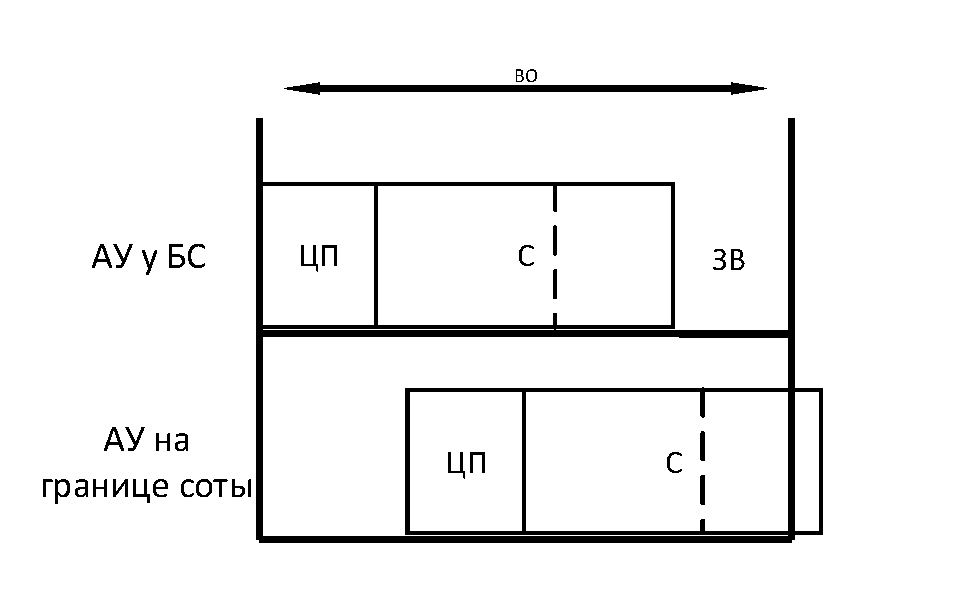
\includegraphics[width=0.8\textwidth]{img/vol_CP}
    \caption{Передача сообщения}
    \label{fig:vol_CP}
\end{figure}

Процесс обмена сообщениями состоит из двух стадий: отправка сообщения и получение ответа
о корректной передаче.
Данная процедура имеет название <<время приема-передачи>> (round-trip delay, RTD) и изображена на
рисунке~\ref{fig:vol_calc_CP}. Таким образом, БС отправляет сообщение АУ и дожидается ответа о том,
что передача произведена корректно.
\begin{figure}[H]
    \centering
    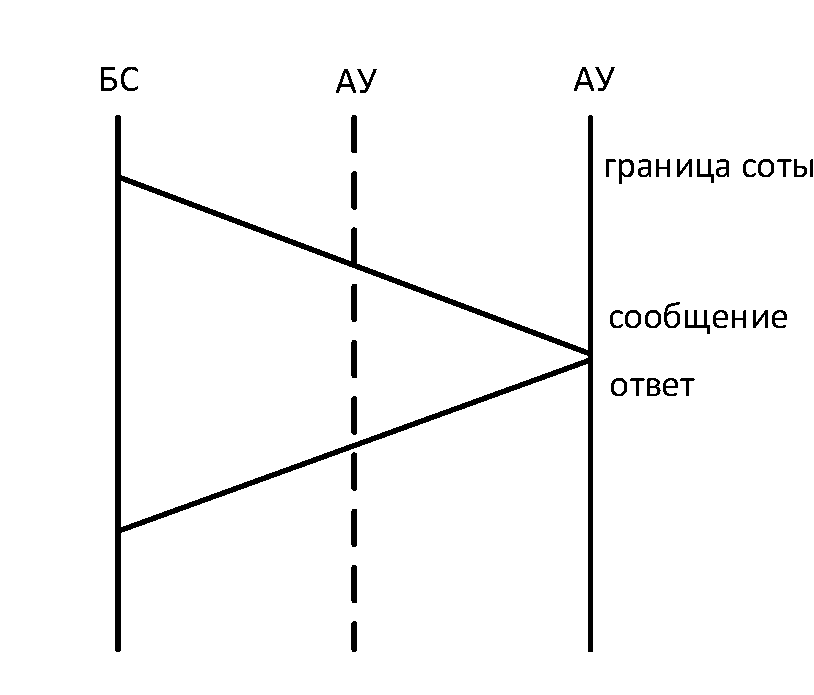
\includegraphics[width=0.5\textwidth]{img/vol_calc_CP}
    \caption{Передача сообщения от БС к АУ на границе соты}
    \label{fig:vol_calc_CP}
\end{figure}

Известно, что сообщение передается со скоростью \(c = 3 \cdot 10^{8} m/s\). Таким образом, время распространения сигнала от БС до дальнего АУ равно \(T = \dfrac{Cell Size}{c}\). Такое же время
распространения ответа от АУ до БС. Отсюда следует, что <<время приема-передачи>> считается как
\[T_{GT} = 2 \cdot T = \dfrac{2 \cdot Cell Size}{c}\]

Как уже говорилось ранее, ЦП и ЗВ идентичны. Отличия данных интервалов в том, что ЦП учитывает
задержку отраженных сигналов (d). Таким образом, расчет интервала ЦП выполняется так
\[T_{CP} = \dfrac{2 \cdot Cell Size}{c} + d\]